\section{Experiments}
\label{sec:exp}
We choose two state-of-the-art models BERT \cite{devlin2018bert} and ERNIE \cite{sun2019ernie} as our baselines. 

BERT is absolutely a milestone in NLP domain. Lots of NLP tasks achieve great improvements with BERT due to its pre-trained knowledge on natural language, including syntax and semantic features. 
Following the structure of pre-trained language model, some other works such as ERNIE and XLNet \cite{yang2019xlnet} come up to further improve the performance of BERT. 
Since training from scratch %on a large corpus 
is time-consuming, we choose the only two publicly released models pre-trained on Chinese corpus, \textbf{\textit{BERT-Base for Chinese}}\footnote{https://github.com/google-research/bert}  and \textbf{\textit{ERNIE 1.0 Base for Chinese}}\footnote{https://github.com/PaddlePaddle/ERNIE} as our baselines, 
%as they are the only two publicly released models pre-trained on the Chinese corpus,
where BERT is trained on Chinese wikipedia and ERNIE is trained on Chinese Wikepedia, Baidu Baike, Baidu news and Baidu Tieba. 
% trained dataset these two models use
%On the basis of BERT, ERNIE further modeled entity and word information to integrate knowledge to some extent.
As these two models are pre-trained using large corpus, we %first 
suppose that they have implicitly learned common sense.%\JQ{commonsense, finetune分分合合}

For our task, we calculate perplexity of phrase $\{w_1, w_2, ..., w_m\}$ %using the pre-trained language model 
by applying the following formula:
\begin{equation}
\label{ppl}
\begin{split}
&perplexity(phrase) = p(w_1, w_2, ..., w_m)^{-1/m} \\
&\approx \sqrt[m]{\prod_{i=1}^{m}\frac{1}{p(w_i|w_1,...,w_{i-1},w_{i+1},..., w_m)}}
\end{split}
\end{equation}
and we choose the one with higher score as the commonsense contradiction phrase.



\subsection{Fine-tune using E-commerce data}
Our dataset are collected from user query on an E-commerce platform. Although the data cover numerous scenarios in daily life, the word distribution is different from Chinese Wikipedia that used in the pre-training process of BERT and ERNIE. Therefore, we use the E-commerce data to fine-tune the model. The details of data used are shown in the Table \ref{tab:DetailData}.

As the training process are very slow due to the large data size, we only conduct the fine-tune process on BERT.% model.

\begin{table}
	\small
	\centering
	\begin{tabular}{cc}
		\toprule[1.1pt]
		Data source & Data Size \\
		\hline
		XiaoHongShu\tablefootnote{XiaoHongShu: https://www.xiaohongshu.com/} & 15 millions \\
		Baidu Baike & 10 millions \\
		Tao GongLue\tablefootnote{Tao GongLue and E-commerce descriptions are both from Taobao: https://www.taobao.com/} & 6+ millions \\
		E-commerce descriptions & 3+ millions \\
		\bottomrule[1.1pt]
	\end{tabular}
	\caption{Details of E-commerce data used for fine tune}
	\label{tab:DetailData}
\end{table}
%\footnotetext[7]{XiaoHongShu: https://www.xiaohongshu.com/}
%\footnotetext[8]{Tao GongLue and E-commerce descriptions are both from Taobao: https://www.taobao.com/}

\subsection{Fine-tune using CoCon dataset}
As we know that, human acquire common sense from his experience or inference based on his knowledge, instead of being told that something is absolutely right. Our released benchmark is also designed to measure if a machine has the commonsense judgment. Hence, we argue that common sense of machine should be learned implicitly from large corpus or inferred by knowledge acquired from external knowledge base, instead of tuning on a specific similar training set.
%in ConceptNet or Probase. 
%It should be noticed that the commonsense concerned more about the intrinsic property of things instead of some facts.  

However, we are also curious about how much the pre-trained language model like BERT can learn from short text. Therefore, we split our dataset into train/dev/test set and use train set to fine-tune the basic BERT and ERNIE.

To avoid the statistical clues revealed by word, we count frequency of each word that appears in either positive or negative side for each sample. Those words, which appear 1.5 times on one class more than another class, will not be put into the train set and test set simultaneously.
%Those words that have obvious statistical feature will not appear in the train set and test set simultaneously.
Finally, the data size of our train/dev/test set are 8343/454/432. %The results of fine-tuned BERT/ERNIE using all CoCon training data are shown in Table \ref{tab:ExpRes}. Besides, the learning curves with varying amounts of  training data will be presented and discussed in the last part of this section.  

For both BERT and ERNIE, we fine tune the network by adding a fully-connected layer over the first token obtained by the last layer in the original model, which is shown in Figure~\ref{fig:tuneNet}, where $S$ is the score obtained by fully-connected layer after softmax function. Because our task needs to compare two phrases in a data sample, hinge loss $L$ is used to do the optimization with threshold $\gamma$ equals to $0.5$. Initial learning rate of both models are set to be %$2e-5$
$2\mathrm{e}{-5}$, and the training epoch is 3. Other parameters are the same as the default settings given by the official tutorial.

\begin{figure}[h!]
	\centering
	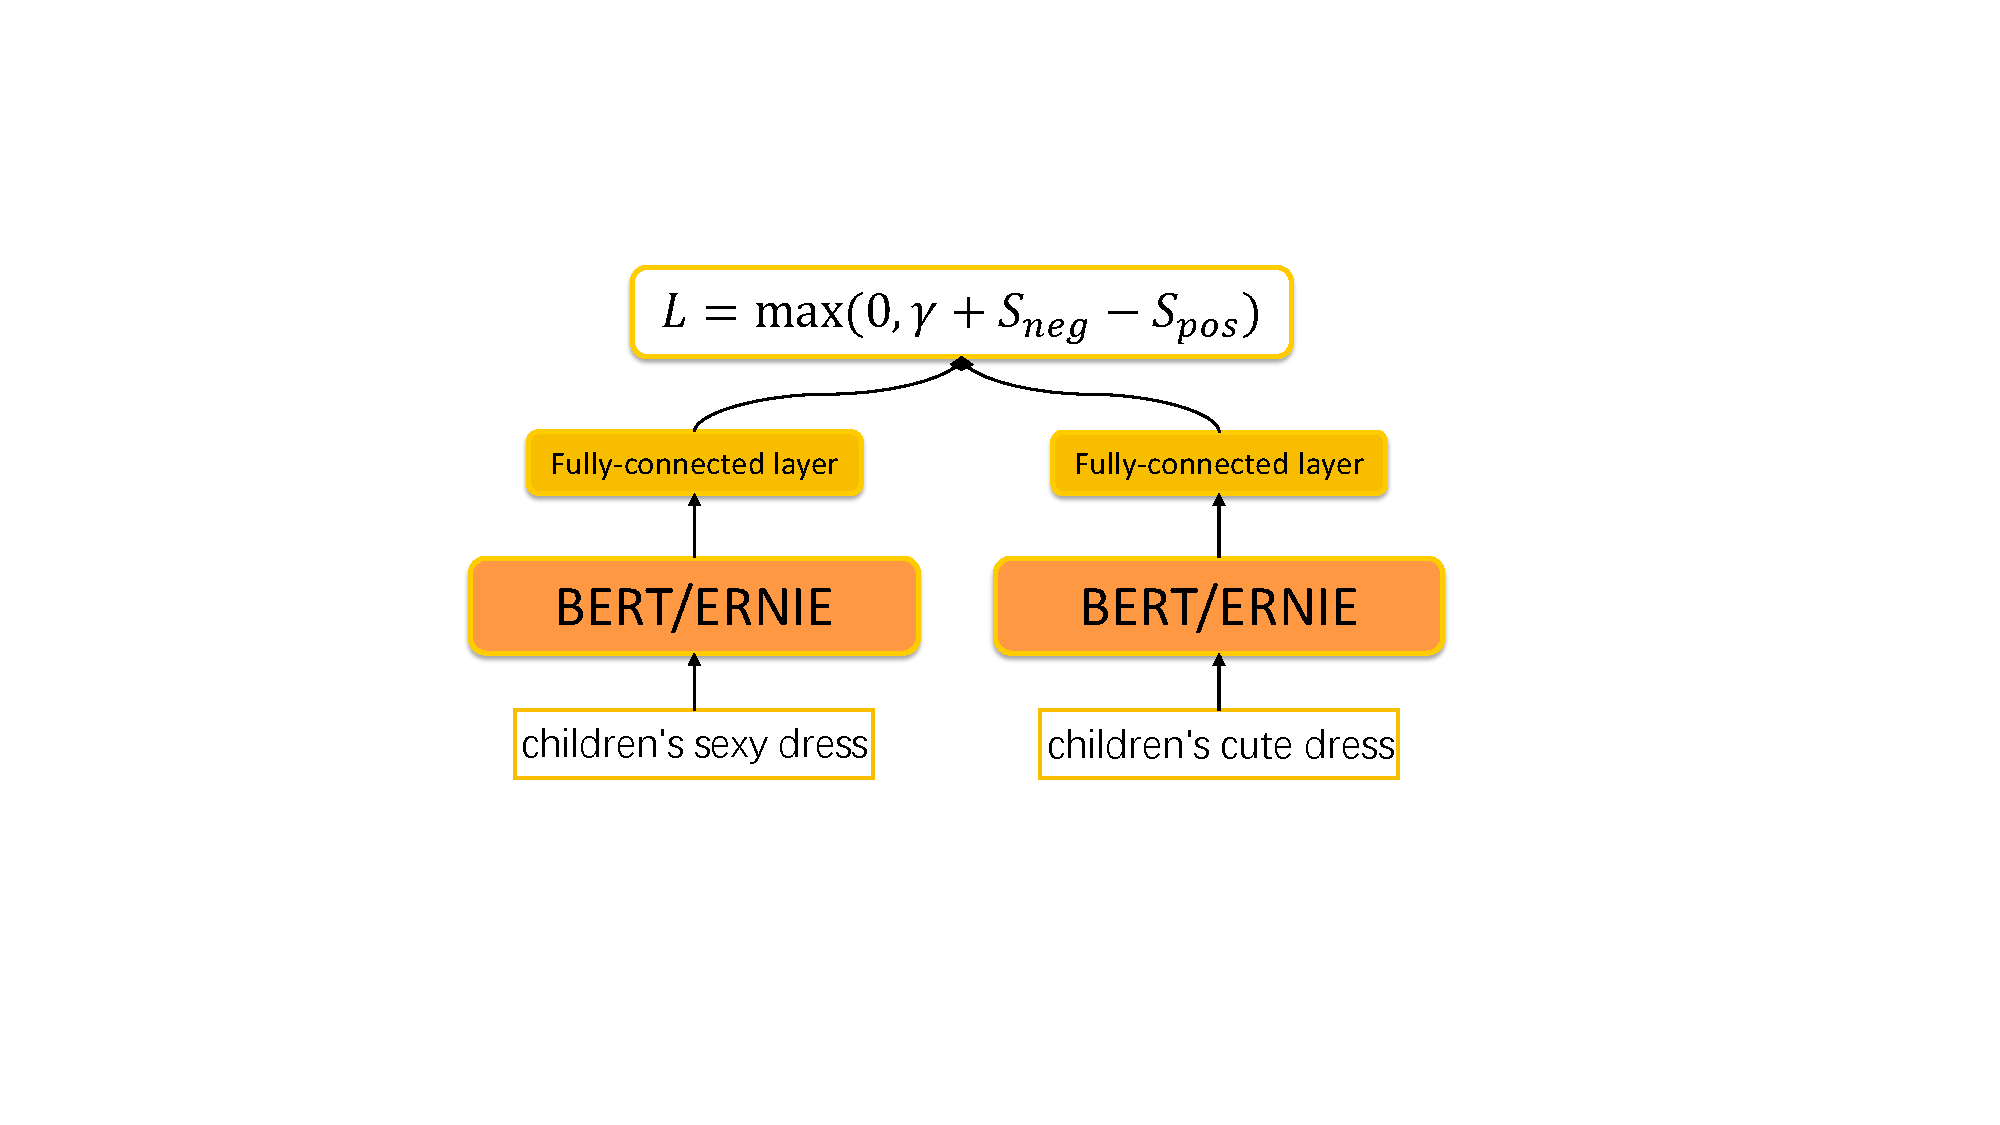
\includegraphics[width=0.8\columnwidth]{images/fineTuneNetwork.pdf}
	\caption{Model of Fine-tuned BERT\&ERNIE}
	\label{fig:tuneNet}
\end{figure}
%\KZ{translate the chinese in the figure to English.}
%\subsection{Experimental Setup}


\subsection{Human Evaluation}
We also conduct human evaluation on our dataset. 100 samples are randomly selected from dataset and distributed to two people, who did not participate in the construction or quality verification process of the dataset. The average of their accuracy are considered as the human performance borderline. 
%Results of experiments are shown in Table \ref{tab:ExpRes}.


\subsection{Results \& Analysis}
Results of all models are shown in Table \ref{tab:ExpRes}. As this is a binary classification problem, the random selection can achieve 50\% accuracy rate. 
The best baseline evaluated on CoCon dataset achieves accuracy of 0.6447. When fine-tuned on CoCon train set is permitted, the best baseline can achieve accuracy of 0.7662 on CoCon test data. However, these two results are both far below the human performance (0.95), demonstrating that our released benchmark is much easier for human, but still remains a great challenge for current state-of-the-art machine. Notice that all results surpass the random choice (0.5), showing that the pre-trained model %can indeed 
try to memorize numerous amounts of information.

\begin{table}
	\small
	\centering
	\begin{tabular}{p{4.3cm}p{1.4cm}p{1.4cm}}
		\toprule[1.1pt]
		Models & Accuracy (CoCon) & Accuracy (CoCon testset) \\
		%Models & Accuracy on CoCon & Accuracy on CoCon testset\\
		\midrule[0.75pt]
		Random & 0.5 & 0.5\\
		%\hline
		BERT & 0.5992 & 0.6019\\
		ERNIE & 0.6007 & 0.6944\\
		Fine-tuned BERT (E-commerce)  & \textbf{0.6447} & 0.6667\\
		Fine-tuned BERT (CoCon) & - & 0.7471\\ %0.7719\\
		Fine-tuned ERNIE (CoCon) & - & \textbf{0.7662} \\ %0.7847\\
		\midrule[0.75pt]
		Human&0.95&0.95\\
		\bottomrule[1.1pt]
	\end{tabular}
	\caption{Accuracy of models on CoCon dataset}
	\label{tab:ExpRes}
\end{table}


Without seeing any related data in CoCon train set and evaluated on the whole CoCon dataset, the basis pre-trained language model BERT (0.5992) and ERNIE (0.6007) perform nearly the same. 
The gap between these two models is considered due to the different size of pre-training data. As BERT uses only Chinese Wikipedia data, and ERNIE uses %another 
additional three data sources (include Baidu Baike/news/Tieba).  Except for Chinese Wikipedia, ERNIE may have seen more relation statistics between words. We also find that the accuracy of BERT improves after fine-tuning using E-commerce data, indicating that the dataset with more similar domain knowledge could further improve models' performance.

Despite of this small improvement, the performance of fine-tuned BERT using E-commerce data is still far from human. We argue that current design of pre-trained language model like BERT or ERNIE can not exactly learn commonsense knowledge from large amounts of training data, it needs to integrate external knowledge in some ways to be further %evaluated 
improved on our released benchmark. Besides, context-poor text also makes the task more challenging for machine to identify the contradiction.
%Besides, our dataset aimed at short text which also makes it more difficult for machine to understand directly as it is absent of enough context and standard syntactic structure.

%the fine-tuned BERT by E-commerce data achieves 

Take the split CoCon data into training process, both BERT and ERNIE get further improvement. The influence of varying amounts of training examples is shown in Section \ref{subsec:lr-curve}. %sub-section.   


%\subsection{Baseline Analysis}

\subsection{Learning Curves}
\label{subsec:lr-curve}

%To better understand the learning performance of both BERT and ERNIE, we fine-tune these two models on different size of CoCon training data.

To extrapolate how current two models BERT and ERNIE perform with various amount of data, we fine tune these two models by varying size of training set. We keep the number of training epochs, initial learning rate and the other hyper-parameters unchanged all the time. To deal with learning stabilities, each data point is the average of 4 runs. The resulting learning curves are plotted in Figure~\ref{fig:learnCurve}. 

We observe that the pre-trained ERNIE performs much better than BERT when the training samples are few, but their performance are getting close with increasing training data. 
The possible reason is that ERNIE tries to mask the entity and the whole word during its language model pre-training process, which may help ERNIE to better learn the relation between words. However the BERT only regard each Chinese character as a mask unit during pre-training. 

%The possible reason is that ERNIE use more training data during pre-trained process, may memorize more relation statistics between words. %However, ERNIE still defeats BERT little  

After using nearly 90\% of total dataset, these two models can merely achieve around 0.75, which is still substantially lower than human performance. Along the tendency of learning curves, large amounts of training samples are needed to approach human, neglecting the training convergence.
% We hypothesize that they will plateau quickly. (no instance)

%However, we hypothesize that both models need very large associated training data to 

\begin{figure}[h!]
	\centering
	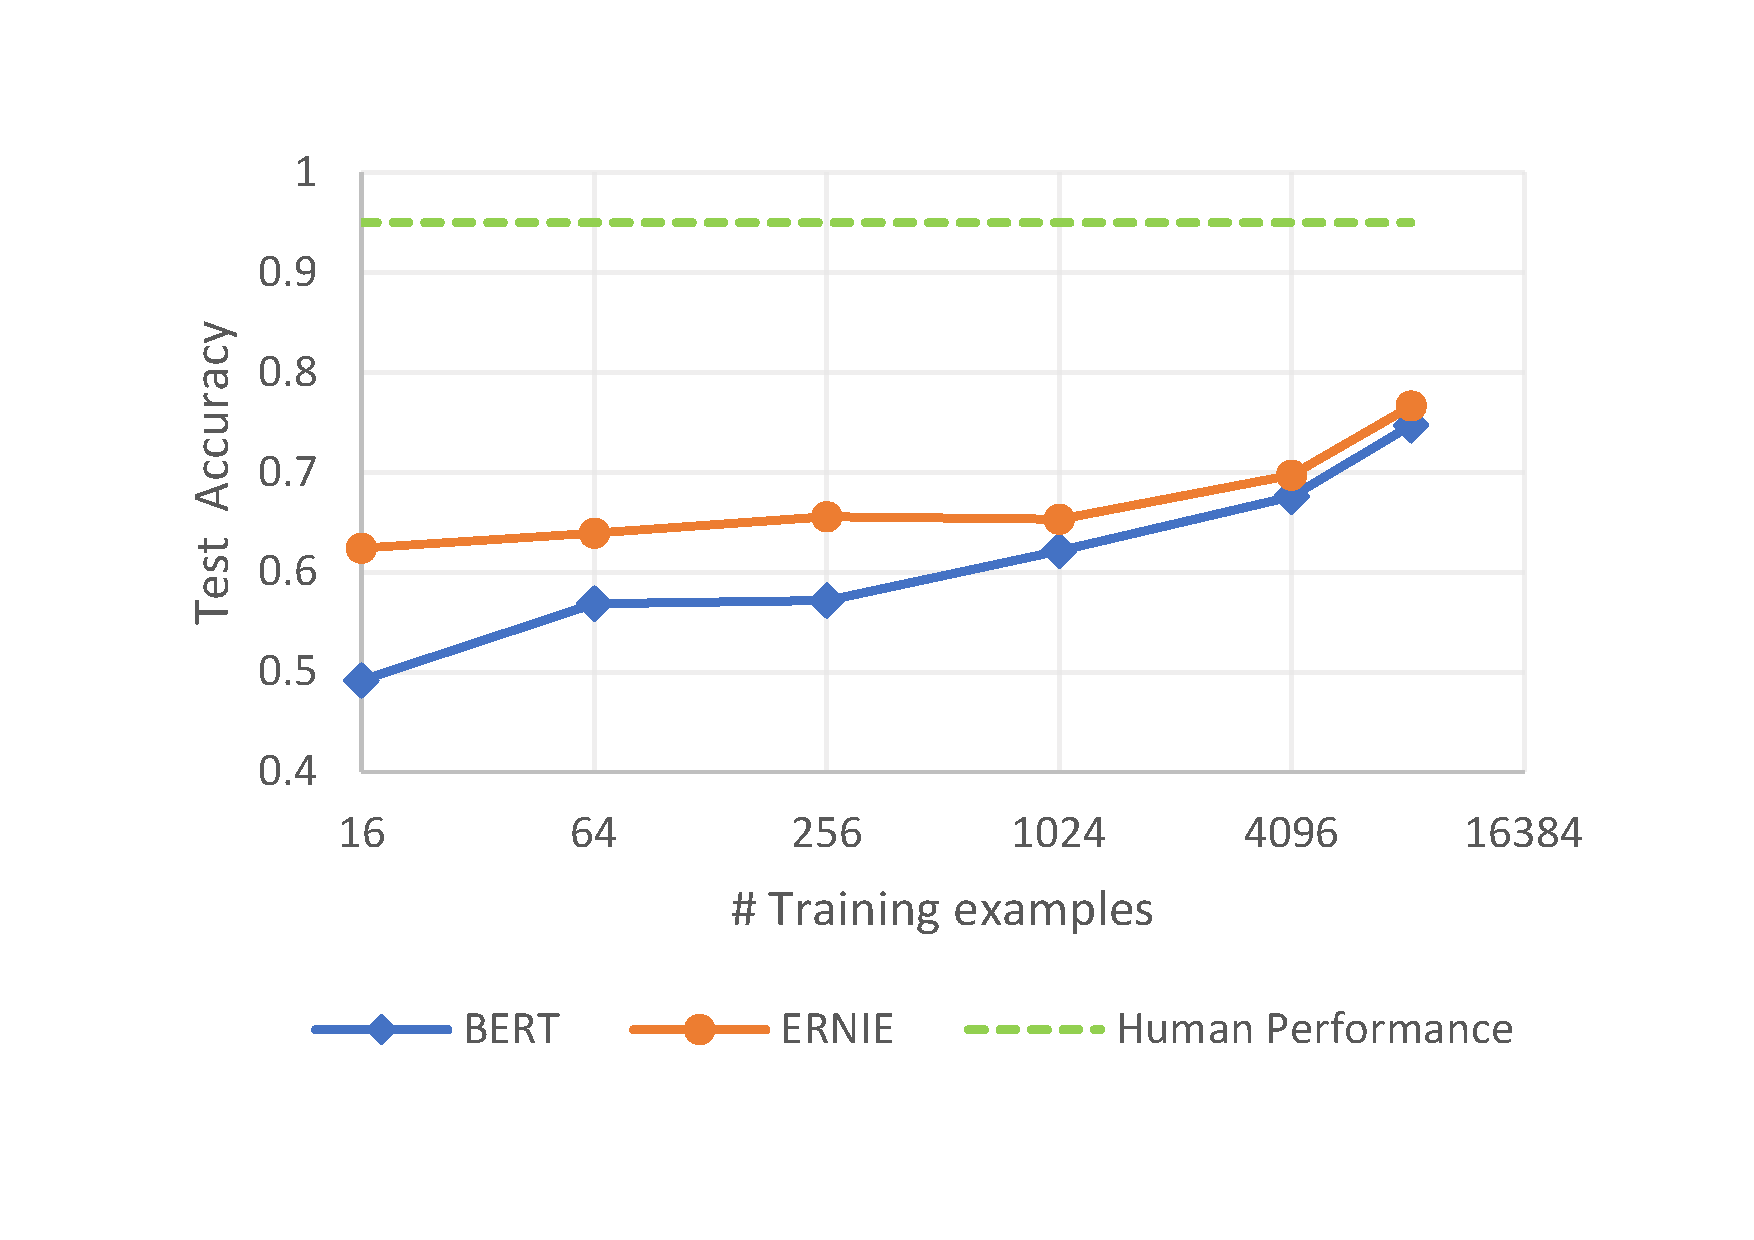
\includegraphics[width=0.85\columnwidth]{images/learnCurveLine.pdf}
	\caption{Accuracy on CoCon test set for BERT/ERNIE fine-tuned with varying amounts of data}
	\label{fig:learnCurve}
\end{figure}

